\exercisesheader{}

% 25 - tf_chisq_1

\eoce{\qt{True or false, Part I\label{tf_chisq_1}} Determine if the statements below 
are true or false. For each false statement, suggest an alternative wording to 
make it a true statement.
\begin{parts}
\item The chi-square distribution, just like the normal distribution, has two 
parameters, mean and standard deviation.
\item The chi-square distribution is always right skewed, regardless of the 
value of the degrees of freedom parameter.
\item The chi-square statistic is always greater than or equal to 0.
\item As the degrees of freedom increases, the shape of the chi-square 
distribution becomes more skewed.
\end{parts}
}{}

% 26 - tf_chisq_2

\eoce{\qt{True or false, Part II\label{tf_chisq_2}} Determine if the statements below 
are true or false. For each false statement, suggest an alternative wording to 
make it a true statement.
\begin{parts}
\item As the degrees of freedom increases, the mean of the chi-square 
distribution increases.
\item If you found $\chi^2 = 10$ with $df = 5$ you would fail to reject $H_0$ 
at the 5\% significance level.
\item When finding the p-value of a chi-square test, we always shade the tail 
areas in both tails.
\item As the degrees of freedom increases, the variability of the chi-square 
distribution decreases.
\end{parts}
}{}

% 27 - opensource_text_chisq_GOF

\eoce{\qt{Open source textbook\label{opensource_text_chisq_GOF}} \videosolution{ahss_eoce_sol-opensource_text_chisq_GOF} A professor using 
an open source introductory statistics book predicts that 60\% of the 
students will purchase a hard copy of the book, 25\% will print it out from 
the web, and 15\% will read it online. At the end of the semester he asks his 
students to complete a survey where they indicate what format of the book 
they used. Of the 126 students, 71 said they bought a hard copy of the book, 
30 said they printed it out from the web, and 25 said they read it online.
\begin{parts}
\item State the hypotheses for testing if the professor's predictions were 
inaccurate.
\item How many students did the professor expect to buy the book, print the 
book, and read the book exclusively online?
\item List the conditions required for the chi-square goodness of fit test and discuss whether they are satisfied.
\item Assume conditions are sufficiently met.  Calculate the chi-square statistic, the degrees of freedom associated 
with it, and the p-value.
\item Based on the p-value calculated in part (d), what is the conclusion of 
the hypothesis test? Interpret your conclusion in this context.
\end{parts}
}{}

% 28 - barking_deer_chisq_GOF_ahss

\eoce{\qt{Barking deer\label{barking_deer_chisq_GOF_ahss}}
Microhabitat factors associated with forage and bed sites
of barking deer in Hainan Island, China were examined.
In this region woods make up 4.8\% of the land,
cultivated grass plot makes up 14.7\%, and deciduous forests
make up 39.6\%.
Of the 426 sites where the deer forage, 4 were categorized
as woods, 16 as cultivated grassplot, and 61 as deciduous forests.
The table below summarizes these data.\footfullcite{Teng:2004}
\begin{center}
\begin{tabular}{c c c c c}
Woods	& Cultivated grassplot	& Deciduous forests	 & Other & Total \\
\hline 
4		& 16					& 61			     & 345	 & 426 \\
\end{tabular}
\end{center}

\noindent \begin{minipage}[c]{0.7\textwidth}
\begin{parts}
\item Do these data provide convincing evidence that barking deer prefer to 
forage in certain habitats over others? Conduct an appropriate hypothesis 
test to answer this research question, and acknowledge any assumptions you had to make to carry out this test.  Include all steps of the Identify, Choose, Check, Calculate, Conclude framework.
\item Interpret the calculated p-value in the context of the problem.
\end{parts}

\end{minipage}
\begin{minipage}[c]{0.03\textwidth}
$\:$ \\
\end{minipage}
\begin{minipage}[c]{0.28\textwidth}
\begin{center}
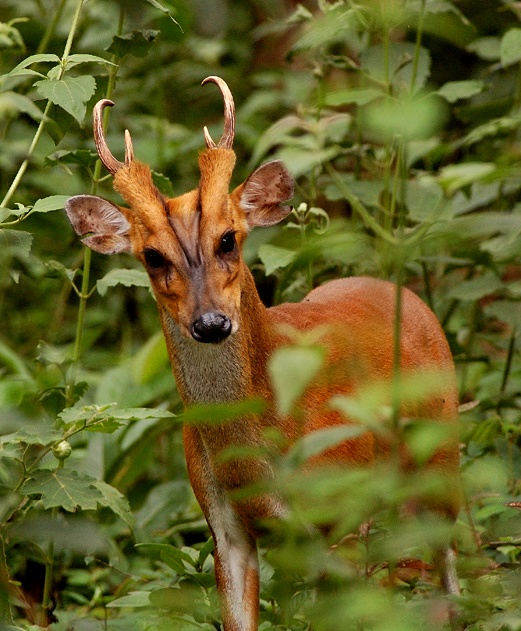
\includegraphics[width=0.7\textwidth]{ch_inference_for_props/figures/eoce/barking_deer_chisq_GOF_ahss/barking_deer.jpg} \\
{\footnotesize Photo by Shrikant Rao (\oiRedirect{textbook-flickr_shrikant_rao_barking_deer}{http://flic.kr/p/4Xjdkk}) \oiRedirect{textbook-CC_BY_2}{CC~BY~2.0~license}}
\end{center}
\end{minipage}
}{}
